A commonly used parameter for quantifying the narrowness of the array main lobe is the Half-Power-Beam-Width (HPBW), marking the DOA where the beampattern's energy reduces to half of its maximal value. 
\par For the passive ULA case, it is known \cite{VanTrees2002DetectionIV} that 
$$
u_{\text{HPBW}} \doteq \frac{\lambda\dTheta_{\text{HPBW}}}{2\pi{}d} = \frac{\lambda}{\pi{}Nd}1.4,
$$
where $\lambda$ is the signal wavelength, linking the HPBW to the array physical aperture $Nd$.
\myTodo{inline}{\textbf{DONE:}\\maybe you can also express this last equation in terms of the electric phase $\theta$, or even better, the error $\Delta\theta$ as well. Then the connection to (12) will be clearer I hope.}
\myTodo{inline}{got up till here with the check. Will continue when I can. Best, Tsvika.}
\ifdefined\DEFIncludeAttenuation
    \par Bearing in mind the tendency of $N\dTheta_{\text{HPBW}}$ towards a finite limit in passive ULA case, we simulate $\Hr{\dTheta}{\dPhi}{}$ for various $\rBrace{N,r,\theta}$ triplets. Investigating  the simulation results lead to the following observations.
    \begin{itemize}
        \item $N\dTheta_{\text{HPBW}}$ tendency towards a finite limit is kept, though the limit value changes for different $r$ values. Figure (\ref{fig_feedbackULA_beamwidth_limit_r_dependent}) shows, for several $r$ values, the tendency of $N\dTheta_{\text{HPBW}}$ with increasing $N$ values. 
        \item Plotting the $\underset{N\to\infty}{lim}N\dTheta_{\text{HPBW}}$ for various $r$ values, and fitting it with $3^{rd}$ order polynomial curve, results in $\underset{N\to\infty}{lim}N\dTheta_{\text{HPBW}} \approx \rBrace{1-r}\rBrace{0.4r^{2}-r+1.4}$ which degenerates to the passive ULA result when setting $r=0$ (i.e. cancelling the feedback).
    \end{itemize}
    \begin{figure}[t!]
        \begin{center}
            \begin{overpic}[width=0.65\linewidth, 
            %grid, 
            tics=10,trim=0 0 0 0]{./Media/spatial_IIR_MATLAB/arrayParameters/HPBW_vs_N_various_r.eps}
                \put (2, 72){\footnotesize{$N\dTheta_{\text{HPBW}}$}}
                \put (50, 62.5) {\footnotesize{$r=0$}}
                \put (50, 54) {\footnotesize{$r=0.1$}}
                \put (50, 39.5) {\footnotesize{$r=0.3$}}
                \put (50, 28.5) {\footnotesize{$r=0.5$}}
                \put (50, 19.75) {\footnotesize{$r=0.7$}}
                \put (50, 12.5) {\footnotesize{$r=0.9$}}
                \put (50, 2) {\footnotesize{$N$}}
            \end{overpic}
        \end{center}
         \caption{Plot of $N\dTheta_{\text{HPBW}}$ vs. N for various $r$ values. In each simulation, $r$ is constant and $\dTheta_{\text{HPBW}}$ is calculated for each $N$ separately and the stored value is $N\dTheta_{\text{HPBW}}$.}
        \label{fig_feedbackULA_beamwidth_Nx_HPBW_1_r_2}
    \end{figure}
    
    \begin{figure}[t!]
        \begin{center}
            \begin{overpic}[width=0.65\linewidth, 
            %grid, 
            tics=10,trim=0 0 0 0]{./Media/spatial_IIR_MATLAB/arrayParameters/HPBW_limit_vs_r.eps}
                \put (40, 61) {\footnotesize{Simulation results}}
                \put (40, 56) {\footnotesize{$\rBrace{1-r}\rBrace{0.4r^{2}-r+1.4}$}}
                \put (-1, 72){\footnotesize{$\underset{N\to\infty}{lim}N\dTheta_{\text{HPBW}}$}}
                \put (50, 2) {\footnotesize{$r$}}
            \end{overpic}
        \end{center}
        \caption{$\underset{N\to\infty}{lim}N\dTheta_{\text{HPBW}}$ vs. $r$ and comparing to $\rBrace{1-r}\rBrace{0.4r^{2}-r+1.4}$}
        \label{fig_feedbackULA_beamwidth_limit_r_dependent}
    \end{figure}
    Following theses two important empirical observations, we formulate the feedback based HPBW expression
    \begin{equation}
            \dTheta_{HPBW} =& \frac{\rBrace{1-r}\rBrace{0.4r^{2}-r+1.4}}{N},
    \end{equation}
    which is naturally translated to the \coefSetName{} feedback related HPBW improvement factor ($\triangleq\mu_{\coefSetName}$)
    \begin{equation}
        \mu_{\text{HPBW},\coefSetName}=\frac{1.4}{\rBrace{1-r}\rBrace{0.4r^{2}-r+1.4}},
    \end{equation}
    stating that a perfectly aligned array (i.e. $r\to1$) will achieve a zero-width spatial beam and an infinite improvement over the classic passive ULA case.
\else
    Defining $\D{N}{x} = \frac{\sin{Nx}}{\sin{x}}$ , and performing some algebraic simplification, one gets
    \ifdefined\showDev
        \\
        \fbox{
        \begin{minipage}{.95\linewidth}
        \textbf{development specifics}
        $$
        \Hr{\theta}{\tau}{}
        =
        \left|
        \frac{
        \vecnot{\alpha}^{T}\vecnot{d}_{\theta_{s}}
        }{
        \vecnot{\alpha}^{T}\vecnot{d}_{\theta}
        }
        \frac{
        1-\vecnot{\beta}^{T}\vecnot{d}_{\theta}e^{-j\tau}
        }{
        1-\vecnot{\beta}^{T}\vecnot{d}_{\theta_{s}}e^{-j\tau_{s}}
        }
        \right|
        =
        \left|
        \frac{
        1
        }{
        \frac{1}{N}\vecnot{d}^{H}_{\theta_{s}}\vecnot{d}_{\theta}
        }
        \frac{
        1-\frac{\rho}{N}\vecnot{d}^{H}_{\theta_{s}}\vecnot{d}_{\theta}e^{j\Delta_{\tau}}
        }{
        1-\rho
        }
        \right|
        $$
        .Using the geometric progression sum of the steering vectors product,
        $$
        \vecnot{d}^{H}_{\theta_{s}}\vecnot{d}_{\theta} = \Sigma_{n=0}^{N-1}e^{j\rBrace{\theta-\theta_{s}}}
        $$
        and defining $\Delta_{\theta} \triangleq \theta-\theta_{s}$ one gets
        $$
        \vecnot{d}^{H}_{\theta_{s}}\vecnot{d}_{\theta} = e^{j\frac{N-1}{2}\Delta_{\theta}}\D{N}{\dTheta}
        $$.
        Integrated into the last expression, it yields\\
        \resizebox{.95\linewidth}{!}{
        \begin{minipage}{\linewidth}
        \begin{align*}
        \left|
        \frac{
        1
        }{
        1-\rho
        }
        \frac{
        N-\rho\vecnot{d}^{H}_{\theta_{s}}\vecnot{d}_{\theta}e^{j\Delta_{\tau}}
        }{
        \vecnot{d}^{H}_{\theta_{s}}\vecnot{d}_{\theta}
        }
        \right|^{2}
        &=
        \left|
        \frac{
        1
        }{
        1-\rho
        }
        \rBrace{
        N\Dp{N}{\dTheta/2}{-1}
        e^{-j\frac{N-1}{2}\Delta_{\theta}}
        - 
        \rho{}e^{j\Delta_{\tau}}
        }
        \right|^{2}
        \\&=
        \left|
        \frac{
        1
        }{
        1-\rho
        }
        \rBrace{
        N\Dp{N}{\dTheta/2}{-1}
        - 
        \rho{}e^{j\rBrace{\Delta_{\tau}+\frac{N-1}{2}\Delta_{\theta}}}
        }
        \right|^{2}
        \\
        &=
        \frac{1}{\left|1-\rho\right|^{2}}
        \rBrace{
        N^{2}\Dp{N}{\dTheta/2}{-2}
        -2rN\Dp{N}{\dTheta/2}{-1}\cos{\rBrace{\Phi+\Delta_{\tau}+\frac{N-1}{2}\Delta_{\theta}}}
        +r^{2}
        }
        \end{align*}
        \end{minipage}}
        \\
        where $ \Delta_{\tau} \triangleq \tau-\tau_{s}$
        \end{minipage}
        }
    \else
    \fi
    \resizebox{.97\linewidth}{!}{
      \begin{minipage}{\linewidth}
          \begin{align}
            \nonumber
            \label{eqn_arrayPerformance_beamwidth_fullEpxr}
            \Hr{\theta}{\tau}{2}
            =
            \frac{1}{\left|1-\rho\right|^{2}}
            \Bigg(
            & 
            N^{2}\Dp{N}{\dTheta/2}{-2} 
            \\ \nonumber &
            - 2rN\Dp{N}{\dTheta/2}{-1}\cos{\rBrace{\Phi+\Delta_{\tau} + \frac{N-1}{2}\Delta_{\theta}}}
            \\ & 
            + r^{2}\Bigg),
        \end{align}
      \end{minipage}
    }
    where $ \Delta_{\tau} \triangleq \tau-\tau_{s} $ and $ \Delta_{\theta} \triangleq \theta-\theta_{s}$.
    which can be easily verified to tend to $ 1 $ when $ \Delta_{\tau},\Delta_{\theta} \rightarrow 0$. 
    Following \cite{VanTrees2002DetectionIV}'s steps (discussed in section \ref{section_arrayPerformance_classicULA}), we start by investigating the first order taylor expansion,$$ \evalat{f\rBrace{x,y}}{x\to{}a,y\to{}b} \approx f(a,b) + \evalat{\frac{\partial{f}}{\partial{x}}}{\rBrace{x=a,x=b}}\rBrace{x-a} + \frac{\partial{f}}{\partial{x}}\rBrace{a,b} $$,of the expression.
    Using L'Hôpital's rule to evaluate the derivatives, results in 
    \resizebox{.97\linewidth}{!}{
      \begin{minipage}{\linewidth}
        \begin{align*}
            \Hr{\theta}{\tau}{2}
            \propto &
            1 
            \\ &
            - \rBrace{r\rBrace{N-1}\sin{\Delta_{\tau}}}\Delta_{\theta}
            \\ &
            -\rBrace{2Nr\mathcal{D}^{-1}\rBrace{N,\sfrac{\Delta}{2}}\sin{\rBrace{\frac{N-1}{2}\frac{\Delta_{\theta}}{2}}}}\Delta_{\tau}.
        \end{align*}
      \end{minipage}
    }
    Observing that setting $\Delta{\tau},\Delta{\theta} = 0$ zeros the first order coefficients, leads us to express the second order terms, resulting in 
    \resizebox{.97\linewidth}{!}{
      \begin{minipage}{\linewidth}
        \begin{align}
            \label{eqn_arrayPerformance_beamwidth_approx}
            \nonumber
            \Hr{\theta}{\tau}{2} 
            \approx 
            1
            +
            \frac{1}{\left|1-\rho\right|^{2}}
            \Bigg(&
            \frac{1}{12}\rBrace{N-1}\rBrace{\rBrace{1+2r}N-4r+1}\Delta^{2}_{\theta}
            \\& \nonumber
            + r\Delta^{2}_{\tau}
            \\&
            + r\rBrace{N-1}\Delta_{\theta}\Delta_{\tau}
            \Bigg).
        \end{align}
      \end{minipage}
    }
    \begin{figure}
        \todo{Refine graph (units , labels, title)}
        \label{fig_singleFreqFeedback_2ndTaylorNumericalValidation}
        \centering
        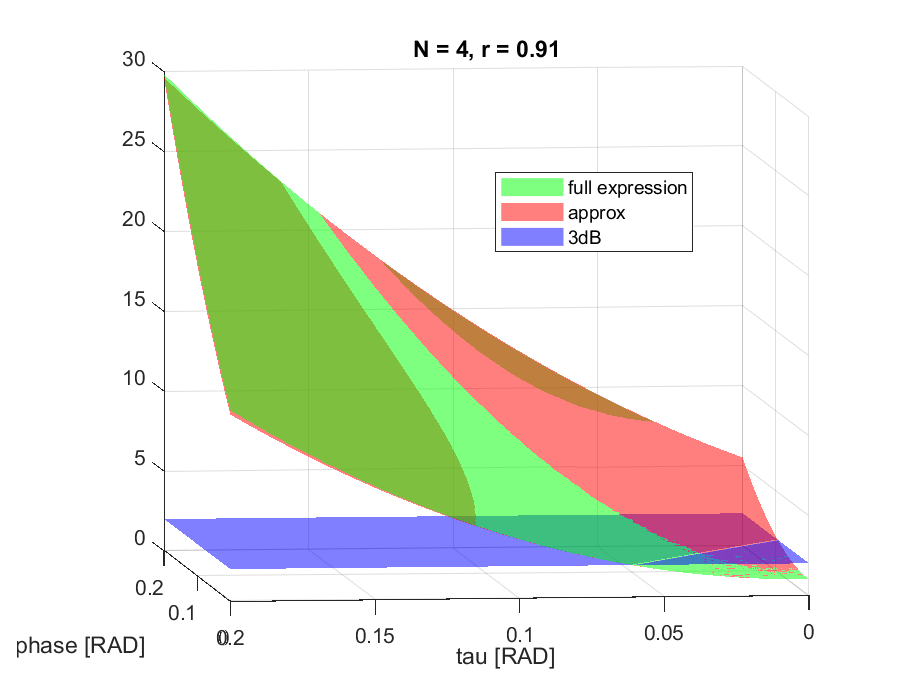
\includegraphics[width=0.9\linewidth]{./Media/spatial_IIR_MATLAB/beamwidth/BW_approx_validation.eps}
        \caption{Graphically comparing (\ref{eqn_arrayPerformance_beamwidth_fullEpxr}) and (\ref{eqn_arrayPerformance_beamwidth_approx}) for $N=4$ and $\rho=0.91$. The approximation seems to closely match the original expression.}
    \end{figure}
    Unlike the passive ULA case, it is evident from figure (\ref{fig_singleFreqFeedback_2ndTaylorNumericalValidation}) that the $4^{th}$ order terms are not needed for the evaluation of $\theta_{\text{HPBW}}$. In perfect phase alignment (i.e. $\Delta_{\tau}=0$), the u-space expression for the HPBW is $$u_{\text{HPBW}} =
    \frac{
    \left|1-\rho\right|
    }{
    \pi{d}
    }
    \lambda
    \sqrt{\frac{
    12
    }{
    \rBrace{N-1}\rBrace{\rBrace{1+2r}N-4r+1}
    }}.
    $$
    Comparing to the classic ULA beamwidth \cite{VanTrees2002DetectionIV}, thoroughly discussed in appendix \ref{appendix_theULABeamwidth}, we can express the improvement factor as
    $$
    \frac{
    0.89\frac{\lambda}{ND}
    }{
    \theta_{\text{HPBW},IIR}
    }
    =
    \frac{0.89}{\left|1-\rho\right|}\sqrt{\frac{1+2r}{12}}
    $$
    \todo{TODO}
    \textbf{Add graph of the improvement factor}
\fi
% \subsection{The pole-based design approach}
% In this approach, we look for setting the response "poles" which minimize the denominator, thus maximizing the overall response magnitude. To evaluate the beamwidth, we chose to allocate all of the system's poles in a single position such that 
% $
% 1-\vecnot{\beta}^{T}\vecnot{d}_{\theta}e^{-j\tau}
% =
% \rBrace{e^{j\theta}-re^{j\theta_{s}}}^{N}
% $
% where $N$ is the number of array sensors and $r \in \left[0,1}$ enables us to avoid treatment of $\infty$-valued expressions. Next, we look for $\theta$ such that
% $
% \left|\frac{
% \frac
% {
% \vecnot{\alpha}^{T}\vecnot{d}_{\theta_{s}}
% }{
% \vecnot{\beta}^{T}\vecnot{d}_{\theta_{s}}
% }
% }{
% \frac
% {
% \vecnot{\alpha}^{T}\vecnot{d}_{\theta}
% }{
% \vecnot{\beta}^{T}\vecnot{d}_{\theta}
% }
% }\right|
% = \frac{1}{\sqrt{2}}
% $. Assuming that, like in classical IIR filter design theory, the numerator behaviour is significantly "slower" than the denominator's which results in $\vecnot{\alpha}^{T}\vecnot{d}_{\theta} 
% \approx
% \vecnot{\alpha}^{T}\vecnot{d}_{\theta_{s}}$ reults in
% \begin{align*}
%     \left|\frac{
%     \vecnot{\beta}^{T}\vecnot{d}_{\theta}
%     }{
%     \vecnot{\beta}^{T}\vecnot{d}_{\theta_{s}}
%     }\right|
%     &= \frac{1}{\sqrt{2}}
%     \\
%     \left|
%     \frac{
%     \rBrace{e^{j\theta}-re^{j\theta}}^{N}
%     }{
%     \rBrace{e^{j\theta}-re^{j\theta_{s}}}^{N}
%     }
%     \right|
%     &=
%     \left|
%     \frac{
%     \rBrace{1-re^{j\rBrace{\theta_{s}-\theta}}}
%     }{
%     \rBrace{1-r}
%     }
%     \right|^{N}
%     \\
%     &=
%     \left|
%     \frac{
%     1+r^{2}-2r\cos{\rBrace{\theta_{s}-\theta}}
%     }{
%     \rBrace{1-r}^{2}
%     }
%     \right|^{\frac{N}{2}}
%     =
%     \rBrace{\frac{1}{2}}^{\frac{1}{2}}
%     \\
%     \Rightarrow 
%     1+r^{2}-2r\cos{\rBrace{\theta_{s}-\theta}}
%     &=
%     \rBrace{1-r}^{2}2^{\frac{1}{N}}
%     \\
%     \cos{\rBrace{\theta_{s}-\theta}}
%     &=
%     \frac{
%     1+r^{2}-\rBrace{1-r}^{2}2^{\frac{1}{N}}
%     }{
%     2r
%     }
%     \\
%     \Rightarrow
%     \frac{\omega{D\rBrace{cos(\theta_{g,s})-cos(\theta_{g,B})}}}{c}
%     &=
%     cos^{-1}
%     \rBrace{
%     \frac{1+r^{2}-\rBrace{1-r}^{2}2^{\frac{1}{N}}}{2r}
%     }
% \end{align*}.
% Therefore,
% \begin{equation}
%     \theta_{g,B} 
%     &= 
%     cos^{-1}
%     \rBrace{
%     cos(\theta_{g,s})
%     -
%     \frac{c}{\omega{D}}
%     cos^{-1}
%     \rBrace{
%     \frac{1+r^{2}-\rBrace{1-r}^{2}2^{\frac{1}{N}}}{2r}
%     }
%     }
% \end{equation}
% Few observations can be derived from the $ \theta_{g,B} $:
% \begin{itemize}
%     \item $r\rightarrow{1}$ (i.e. setting the pole on the unit circle) causes $\theta_{g,B}\rightarrow\theta_{g,s}$ due to the $\infty$ valued response at $\theta_{g,s}$
%     \item The interval 
%     $
%     \left\{
%     \theta_{g,s}
%     \ \Bigg{|}\ 
%     cos(\theta_{g,s})
%     -
%     \frac{c}{\omega{D}}
%     cos^{-1}
%     \rBrace{
%     \frac{1+r^{2}-\rBrace{1-r}^{2}2^{\frac{1}{N}}}{2r}
%     }
%     <-1
%     \right\}
%     $, has no solution. In simulations, when evaluating such $\theta_{g,s}$ values, one can observe that the actual beampattern does not resemble the designed one due to the ULA geometric properties.
%     \item The number of sensors $N$ seems to have low impact on the beamwidth.
% \end{itemize}